\documentclass[./main.tex]{subfiles}

\begin{document}
\onehalfspacing
\section{Ենթաբազմության վրա մակածված տոպոլոգիան և նրա հատկությունները. տոպոլոգիական տարածության ենթատարածության հասկացությունը։ Ենթատարածությունների օրինակներ։}\label{sec:12}

\par Դիցուք ունենք $(X,\tau)$ տոպոլոգիական տարածություն և $A \subset X$ են\-թա\-բազ\-մու\-թյուն։ Այդ ենթաբազմությունը վերածվում է տոպոլոգիական տարածության, որի $\tau_A$ տոպոլոգիան կազմվում է $A$-ի այն բոլոր ենթաբազմություններով, որոնք ստացվում են $A$-ի հետ $X$-ում բաց բոլոր $U_i$ ենթաբազմությունների հատումներից՝\\
$\tau_A =\{U_i \cap A\mid U_i \in \tau \}$։
\par Այսպիսով, \textbf{ըստ սահմանման}, $A$ բազմությունում բաց ենթաբազմություններ են համարվում $X$-ում բաց բազմությունների հատումները $A$-ի հետ։
\par Ցույց տանք, որ $\tau_A$-ի համար տոպոլոգիայի 1-3 աքսիոմները բավարարվում են։
Իրոք,
\begin{enumerate}
    \item $\varnothing \cap A= \varnothing,\ X \cap A=A$, ուստի $\varnothing$-ը և $A$-ն պատկանում են $\tau_A$-ին։
    \item Քանի որ $\bigcup\limits_i (U_i \cap A)=\Big(\bigcup\limits_i U_i\Big) \cap A$, ուստի  $\tau_A$-ի ցանկացած քանակով $U_i \cap A$ տարրերի միավորումը (որտեղ $U_i \in \tau$) նույնպես պատկանում է $\tau_A$-ին։
    \item Քանի որ $\bigcap\limits_{i=1}^n(U_i \cap A)=\Big(\bigcap\limits_{i=1}^n U_i\Big) \cap A$, ուստի հատման աքսիոմը ևս տեղի ունի։ 
\end{enumerate}
% 5
\begin{definition}
$\tau_A$ տոպոլոգիան կոչվում է $\tau$ տոպոլոգիայից \textbf{մակածված տո\-պո\-լո\-գիա} $A$ ենթաբազմության վրա։ Իսկ ինքը՝ $(A, \tau_A)$  տոպոլոգիական տարածությունը կոչվում է $(X, \tau)$ \textbf{տոպ. տարածության ենթատարածություն}։\par Մասնավոր $A=X$ դեպքում $\tau_A=\tau$, և ունենք $(A,\tau_A)=(X,\tau)$ նույնացում։
\end{definition}
% 6
\par Սահմանումից հետևում է, որ $(A, \tau_A)$ տարածության փակ ենթաբազմությունները ստացվում են $A$-ի հետ $X$-ում փակ ենթաբազմությունների հատումներով։
% 7
\subsubsection*{Մակածված տոպոլոգիայի հատկություններ։}
\begin{hatkutyun}
Ունենք $(X, \tau)$ տոպ. տարածություն, $A \subset B \subset X$ են\-թա\-բազ\-մու\-թյուն\-ներ։ $A$ ենթաբազմության վրա կարելի է մակածել երկու տոպոլոգիա՝ $\tau_A$ (անմիջականորեն  $\tau$-ից $A$-ի վրա) և ${(\tau_B)}_A$ (նախ $\tau$-ից մակածվում է $\tau_B$ տոպոլոգիա $B$-ի վրա, ապա $\tau_B$-ից մակածվում է տոպոլոգիա $A$-ի վրա՝ ${(\tau_B)}_A$։ Հետևյալ ակնհայտ $U \cap  A= (U \cap B) \cap A$ համընկման շնորհիվ $\tau_A$ և ${(\tau_B)}_A$ տոպոլոգիաները նույնն են։
\end{hatkutyun} 
% 8
\begin{hatkutyun}
Եթե $\{V_i\}$ ընտանիքը բազա է $\tau$ տոպոլոգիայի համար, ապա $\{V_i \cap A\}$ ընտանիքը բազա է $\tau_A$-ի համար։
\par Եթե $\{U_j(x);\, j\in J\}$ ընտանիքը $x\in A$ կետի շրջակայքերի բազա է $(X,\tau)$ տարա\-ծությունում, ապա $\{U_j(x)\cap A;\, j\in J\}$ ընտանիքը $x$ կետի շրջակայքերի բազա է $(A,\tau_A)$ տարածությունում։
\end{hatkutyun} 

% 9
\begin{example}
$(\mathbb{R}, \textrm{սովոր.})$ տարածության $A=[a,b]$ ենթաբազմության $\tau_A$ տո\-պո\-լո\-գիա\-յի համար բազա են կազմում հետևյալ երեք տեսքերի ենթաբազմությունները, որոնք գոյանում են ինտերվալների $(\alpha,\beta) \cap A$ հատումներով.
\renewcommand\windowpagestuff{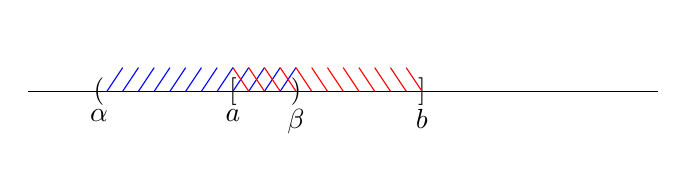
\begin{tikzpicture}
    \def\x{4}
    \def\tick{0.25}
    \def\vx{0.2}
    \def\vy{0.3}
    
    % 1-ին գծագիրն ա
    \begin{scope}[xshift=6cm, yshift=0.3cm]
    \draw[white] (0,0) -- (0,0.5);
    \end{scope}
    \begin{scope}[xshift=6cm]
    \draw (-1,0) -- (\x+3,0);
    \node (lpakagic) at (-0.1,0) {$($};
    \node[below=3pt] at (lpakagic) {$\alpha$};
    \node (rpakagic) at (0.6*\x,0) {$)$};
    \node[below=3pt] at (rpakagic) {$\beta$};
    \node (left) at (0.4*\x, 0) {$[$};
    \node[below=3pt] at (left) {$a$};
    \node (right) at (\x, 0) {$]$};
    \node[below=3pt] at (right) {$b$};
    % blues
    \draw[blue] (0, 0) -- (\vx,\vy);
    \draw[blue] (0.05*\x, 0) -- (0.05*\x+\vx,\vy);
    \draw[blue] (0.1*\x, 0) -- (0.1*\x+\vx,\vy);
    \draw[blue] (0.15*\x, 0) -- (0.15*\x+\vx,\vy);
    \draw[blue] (0.2*\x, 0) -- (0.2*\x+\vx,\vy);
    \draw[blue] (0.25*\x, 0) -- (0.25*\x+\vx,\vy);
    \draw[blue] (0.3*\x, 0) -- (0.3*\x+\vx,\vy);
    \draw[blue] (0.35*\x, 0) -- (0.35*\x+\vx,\vy);
    \draw[blue] (0.4*\x, 0) -- (0.4*\x+\vx,\vy);
    \draw[blue] (0.45*\x, 0) -- (0.45*\x+\vx,\vy);
    \draw[blue] (0.5*\x, 0) -- (0.5*\x+\vx,\vy);
    \draw[blue] (0.55*\x, 0) -- (0.55*\x+\vx,\vy);
    % reds
    \draw[red] (\x,0) -- (\x-\vx, \vy);
    \draw[red] (0.95*\x,0) -- (0.95*\x-\vx, \vy);
    \draw[red] (0.9*\x,0) -- (0.9*\x-\vx, \vy);
    \draw[red] (0.85*\x,0) -- (0.85*\x-\vx, \vy);
    \draw[red] (0.8*\x,0) -- (0.8*\x-\vx, \vy);
    \draw[red] (0.75*\x,0) -- (0.75*\x-\vx, \vy);
    \draw[red] (0.7*\x,0) -- (0.7*\x-\vx, \vy);
    \draw[red] (0.65*\x,0) -- (0.65*\x-\vx, \vy);
    \draw[red] (0.6*\x,0) -- (0.6*\x-\vx, \vy);
    \draw[red] (0.55*\x,0) -- (0.55*\x-\vx, \vy);
    \draw[red] (0.5*\x,0) -- (0.5*\x-\vx, \vy);
    \draw[red] (0.45*\x,0) -- (0.45*\x-\vx, \vy);
    \end{scope}
\end{tikzpicture}}%

\begin{cutout}{0}{7cm}{0pt}{1}
ա) $[a,\beta)$, որտեղ $a<\beta\leq b$\\
\\ \\
\end{cutout}

\renewcommand\windowpagestuff{
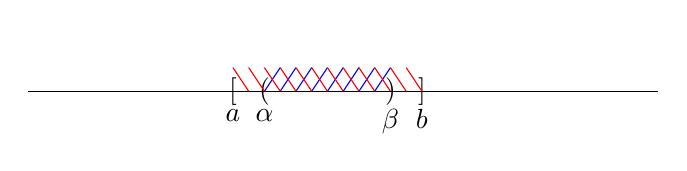
\begin{tikzpicture}
    \def\x{4}
    \def\tick{0.25}
    \def\vx{0.2}
    \def\vy{0.3}

% 2-րդ գծագիրն ա
    \begin{scope}[xshift=6cm, yshift=0.3cm]
    \draw[white] (0,0) -- (0,0.5);
    \end{scope}
    \begin{scope}[xshift=6cm]
    \draw (-1,0) -- (\x+3,0);
    \node (lpakagic) at (0.9*\x,0) {$)$};
    \node[below=3pt] at (lpakagic) {$\beta$};
    \node (rpakagic) at (0.5*\x,0) {$($};
    \node[below=3pt] at (rpakagic) {$\alpha$};
    \node (left) at (0.4*\x, 0) {$[$};
    \node[below=3pt] at (left) {$a$};
    \node (right) at (\x, 0) {$]$};
    \node[below=3pt] at (right) {$b$};
    % blues
    \draw[blue] (0.5*\x, 0) -- (0.5*\x+\vx,\vy);
    \draw[blue] (0.55*\x, 0) -- (0.55*\x+\vx,\vy);
    \draw[blue] (0.6*\x, 0) -- (0.6*\x+\vx,\vy);
    \draw[blue] (0.65*\x, 0) -- (0.65*\x+\vx,\vy);
    \draw[blue] (0.75*\x, 0) -- (0.75*\x+\vx,\vy);
    \draw[blue] (0.7*\x, 0) -- (0.7*\x+\vx,\vy);
    \draw[blue] (0.8*\x, 0) -- (0.8*\x+\vx,\vy);
    \draw[blue] (0.85*\x, 0) -- (0.85*\x+\vx,\vy);
    % reds
    \draw[red] (\x,0) -- (\x-\vx, \vy);
    \draw[red] (0.95*\x,0) -- (0.95*\x-\vx, \vy);
    \draw[red] (0.9*\x,0) -- (0.9*\x-\vx, \vy);
    \draw[red] (0.85*\x,0) -- (0.85*\x-\vx, \vy);
    \draw[red] (0.8*\x,0) -- (0.8*\x-\vx, \vy);
    \draw[red] (0.75*\x,0) -- (0.75*\x-\vx, \vy);
    \draw[red] (0.7*\x,0) -- (0.7*\x-\vx, \vy);
    \draw[red] (0.65*\x,0) -- (0.65*\x-\vx, \vy);
    \draw[red] (0.6*\x,0) -- (0.6*\x-\vx, \vy);
    \draw[red] (0.55*\x,0) -- (0.55*\x-\vx, \vy);
    \draw[red] (0.5*\x,0) -- (0.5*\x-\vx, \vy);
    \draw[red] (0.45*\x,0) -- (0.45*\x-\vx, \vy);
    \end{scope}
    \end{tikzpicture}
}

\begin{cutout}{0}{7cm}{0pt}{1}
բ) $(\alpha,\beta)$, որտեղ $a\leq\alpha<\beta\leq b$\\ \\ \\
\end{cutout}

\renewcommand\windowpagestuff{
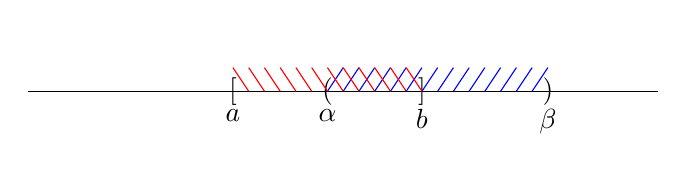
\begin{tikzpicture}
    \def\x{4}
    \def\tick{0.25}
    \def\vx{0.2}
    \def\vy{0.3}

%3-րդ գծագիրն ա
    \begin{scope}[xshift=6cm, yshift=0.3cm]
    \draw[white] (0,0) -- (0,0.5);
    \end{scope}
    \begin{scope}[xshift=6cm]
    \draw (-1,0) -- (\x+3,0);
    \node (lpakagic) at (\x+1.6,0) {$)$};
    \node[below=3pt] at (lpakagic) {$\beta$};
    \node (rpakagic) at (0.7*\x,0) {$($};
    \node[below=3pt] at (rpakagic) {$\alpha$};
    \node (left) at (0.4*\x, 0) {$[$};
    \node[below=3pt] at (left) {$a$};
    \node (right) at (\x, 0) {$]$};
    \node[below=3pt] at (right) {$b$};
    % blues
    \draw[blue] (0.7*\x, 0) -- (0.7*\x+\vx,\vy);
    \draw[blue] (0.75*\x, 0) -- (0.75*\x+\vx,\vy);
    \draw[blue] (0.8*\x, 0) -- (0.8*\x+\vx,\vy);
    \draw[blue] (0.85*\x, 0) -- (0.85*\x+\vx,\vy);
    \draw[blue] (0.9*\x, 0) -- (0.9*\x+\vx,\vy);
    \draw[blue] (0.95*\x, 0) -- (0.95*\x+\vx,\vy);
    \draw[blue] (\x, 0) -- (\x+\vx,\vy);
    \draw[blue] (1.05*\x, 0) -- (1.05*\x+\vx,\vy);
    \draw[blue] (1.1*\x, 0) -- (1.1*\x+\vx,\vy);
    \draw[blue] (1.15*\x, 0) -- (1.15*\x+\vx,\vy);
    \draw[blue] (1.2*\x, 0) -- (1.2*\x+\vx,\vy);
    \draw[blue] (1.25*\x, 0) -- (1.25*\x+\vx,\vy);
    \draw[blue] (1.3*\x, 0) -- (1.3*\x+\vx,\vy);
    \draw[blue] (1.35*\x, 0) -- (1.35*\x+\vx,\vy);
    % reds
    \draw[red] (\x,0) -- (\x-\vx, \vy);
    \draw[red] (0.95*\x,0) -- (0.95*\x-\vx, \vy);
    \draw[red] (0.9*\x,0) -- (0.9*\x-\vx, \vy);
    \draw[red] (0.85*\x,0) -- (0.85*\x-\vx, \vy);
    \draw[red] (0.8*\x,0) -- (0.8*\x-\vx, \vy);
    \draw[red] (0.75*\x,0) -- (0.75*\x-\vx, \vy);
    \draw[red] (0.7*\x,0) -- (0.7*\x-\vx, \vy);
    \draw[red] (0.65*\x,0) -- (0.65*\x-\vx, \vy);
    \draw[red] (0.6*\x,0) -- (0.6*\x-\vx, \vy);
    \draw[red] (0.55*\x,0) -- (0.55*\x-\vx, \vy);
    \draw[red] (0.5*\x,0) -- (0.5*\x-\vx, \vy);
    \draw[red] (0.45*\x,0) -- (0.45*\x-\vx, \vy);
    \end{scope}
    \end{tikzpicture}

}
\begin{cutout}{0}{7cm}{0pt}{1}
գ) $(\alpha,b]$, որտեղ $a\leq\alpha<b$\\ \\
\end{cutout}
\par Այս օրինակը ցույց է տալիս, որ ենթատարածության բաց բազմությունները կարող են բաց չլինել ընդգրկող տարածությունում։ Նկատենք նաև, որ տվյալ $(A, \tau_A)$ են\-թա\-տա\-րա\-ծու\-թյու\-նում փակ են $[a,b]$-ի այն և միայն այն ենթաբազմությունները, որոնք փակ են նաև $(\R,\textrm{սովոր.})$ ընդգրկող տարածությունում։
\end{example}
% 12
\begin{example}
 $B=(0,1) \subset \R$ տոպոլոգիական տարածությունում (որպես $(\mathbb{R}, \textrm{սովոր.})$ տարածության ենթատարածություն) բաց են բոլոր ${(\alpha,\beta),\ 0\leq a<\beta\leq 1}$ տես\-քի ինտերվալներն ու նրանց միավորումները (այսինքն տվյալ են\-թա\-տա\-րա\-ծու\-թյան բաց բազմությունները բաց են նաև ընդգրկող տարածությունում)։ Նկատենք նաև, որ $(0, 1)$-ում փակ են $(0,\beta],\ 0<\beta< 1$ և $ [\alpha,\beta],\ 0<\alpha<\beta< 1$ տեսքերի ենթաբազմու\-թյուն\-ներն ու նրանց վերջավոր միավորումները։ Ուստի $(0, 1)$-ում փակ որոշ ենթա\-բազ\-մություններ փակ չեն ընդգրկող $(\mathbb{R}, \textrm{սովոր.})$ տարածությունում։
\end{example}
Ընդհանուր դեպքում, ենթատարածությունում բաց որևէ ենթաբազմություն կա\-րող է չլինել բաց ենթաբազմություն ընդգրկող տարածությունում և են\-թա\-տա\-րա\-ծու\-թյու\-նում փակ որևէ ենթաբազմություն կարող է փակ չլինել ընդգրկող տա\-րա\-ծու\-թյու\-նում։ Ընթերցողին առաջարկում ենք որպես օգտակար վարժանք քննարկել (նկարագրել) բաց և փակ ենթաբազմություննեը $(\mathbb{R},\textrm{սովոր.})$ տարածության $[0, 1)$ և $(0,1]$ ենթատարածություններում։

\begin{theorem}
Ունենք $(X,\tau)$ տոպ․ տարածություն և $A \subset X$ ենթաբազմություն։ Ապա հետևյալ երկու պնդումները համարժեք են միմյանց.
\begin{enumerate}
    \item $(A, \tau_A)$ ենթատարածության կամայական բաց ենթաբազմություն, բաց են\-թա\-բազ\-մու\-թյուն է նաև $(X, \tau)$ ընդգրկող տարածությունում:
    \item $A$-ն բաց ենթաբազմություն է $X$-ում։
\end{enumerate}
\end{theorem} %թեորեմ 1
\label{թեորեմ 1}
\par Նշենք, որ նմանակ պնդում տեղի ունի նաև փակ ենթաբազմությունների դեպքում․ հարկավոր է \hyperref[թեորեմ 1]{թեորեմ 1}-ի ձևակերպման մեջ ամենուրեք <<բաց ենթաբազմություն>> բառակապակցությունը փոխարինել <<փակ ենթաբազմություն>>-ով։
\begin{proof} 
Ցույց տանք $1\rightarrow 2$ անցումը։ Քանի որ $A$-ն բաց ենթաբազմություն է $(A, \tau_A)$ տարածությունում, ուստի $1$-ից հետևում է, որ $A$-ն բաց ենթաբազմություն է նաև $X$-ում։
Այժմ հակառակը. դիցուք $A$-ն բաց է ենթաբազմության $X$-ում։ Դի\-տար\-կենք կամայական $V$ բաց բազմություն $A$-ում։ Ըստ  $\tau _A$-ի սահմանման $\exists U \in \tau$, որ $V=U \cap A$։ Ուստի $V$-ն բաց է $X$-ում` որպես  $X$-ում բաց երկու ենթաբազմությունների հատում։
\end{proof}
%18
\begin{example}
Դիտարկենք որևէ $S$ շրջանագիծ $\mathbb{R}^2$ կոորդինատային հար\-թու\-թյու\-նում։
%\begin{wrapfigure}{l}{0pt}
%\centering
\begin{center}
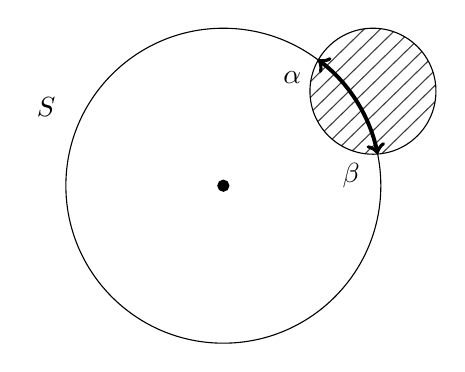
\begin{tikzpicture}
%big circle
\draw (2,2) circle (2cm);
\filldraw (2,2) circle (2pt);
\draw (3.9, 3.2) circle (0.8cm);
\draw[ultra thick, line width=0.5mm, black, <->] (3.959143645958,2.402189227233) arc (11.5:53:2cm);

%adding nodes
\node at (2.875,3.375) {$\alpha$};
\node at (3.625,2.125) {$\beta$};
\node at (-0.25,3) {$S$};

%filling small circle
\draw[opacity=0.75] (3.8,4) -- (3.1100259123993,3.3262574390657);
\draw[opacity=0.75] (3.9992277876714,3.9938223013709) -- (3.104040817744,3.1196944573368);
\draw[opacity=0.75] (4.1609027672357,3.9562603692173) -- (3.1377440073104,2.9571712504484);
\draw[opacity=0.75] (4.3029439474233,3.8911122739721)
-- (3.1994928581483,2.8136196896648);
\draw[opacity=0.75] (4.4213811687039,3.8067632791468)
-- (3.2809989778652,2.693208391352);
\draw[opacity=0.75] (4.5211365723173,3.7041719533392)
-- (3.3811869152492,2.5910394240253);
\draw[opacity=0.75] (4.6021881631104,3.5833168188165)
-- (3.5000786654537,2.5071342654059);
\draw[opacity=0.75] (4.6624640374033,3.4421747131033)
-- (3.6397491321583,2.4435160779809);
\draw[opacity=0.75] (4.695959182256,3.2803055426632)
-- (3.8007722123286,2.4061776989261);
\draw[opacity=0.75] (4.6890589232482,3.068143958643)
-- (4.0130379283083,2.4080262461648);
\end{tikzpicture}
\end{center}
%\end{wrapfigure}

\par Քանի որ $\R^2$-ի մետրական տոպոլոգիայի համար բազա են կազմում անեզր շրջան\-նե\-րը, ուստի (համաձայն հատկություն $1$-ի) $S$-ի մակածված տոպոլոգիայի համար բազա են կազմում շրջանագծի բոլոր անեզր $\alpha\beta$ աղեղները։
\end{example}
% 20
\begin{example}
  $(\mathbb{R}^3,\textrm{սովոր. մետր. տոպ.})$ տարածությունում դիտարկենք $T^2$ տորը (մակերևույթ, որն առաջանում է շրջանագիծն իրեն չհատող ուղղի շուրջ տա\-րա\-ծու\-թյան մեջ պտտումով (տե՛ս նաև թեմա $2$-ում)։ Այս մակերևույթի $\R^3$-ից մակածված տոպոլոգիայի համար բազա են կազմում նրա հատումները անեզր գնդերի հետ։
  
\begin{center}
  \includegraphics[scale=0.075]{images/id19.jpg}
\end{center}
\end{example}
% 21

\begin{example}
Դիտարկենք $(\mathbb{R}^{n+1},\textrm{սովոր. մետր. տոպ.})$ տարածության \\$S^n=\Big\{(x_1,x_2,\dots ,x_{n+1})\mid \sum\limits_{i=1}^{n+1} x_i^2=1\Big\} $ ենթաբազմությունը (այն կոչվում է $\mathbb{R} ^{n+1}$ էվկլիդյան տարածության $n$-չափականության սֆերա)։ Կարելի է $S^n$-ի վրա մակածել տո\-պո\-լո\-գիա  $\mathbb{R} ^{n+1}$-ի մետրական տոպոլոգիայից. նրա համար բազա են կազմում $S^n\textrm{-ի}$ հատումները $\mathbb{R}^{n+1}$-ի $n+1$ չափականության անեզր գնդերի հետ։ Այս օրի\-նակը կարելի է դիտել որպես օրինակ $3$-ի ընդհանրացում։
\end{example}
% 22
\begin{example}
$\mathbb{R}^n$ էվկլիդյան տարածությունը կարելի է դիտել որպես $\mathbb{R}^{n+1}$ էվկլիդյան տարածության ենթատարածություն կազմված բոլոր $(x_1,x_2,\dots,x_n,0)$ կետերից։ Ուս\-տի $\mathbb{R}^n$-ի մետրական տոպոլոգիան համընկնում է $\mathbb{R}^n$-ի վրա $\mathbb{R}^{n+1}$-ի մետրական տո\-պո\-լո\-գիա\-յից մակածված տոպոլոգիայի հետ։ Նկատենք, որ  $\mathbb{R}^n$-ը փակ ենթաբազմություն է $\mathbb{R}^{n+1}$-ում (ինչո՞ւ)։ Ուստի (համաձայն փակ ենթաբազմության վերաբերյալ \hyperref[թեորեմ 1]{թեորեմ 1}-ի նմանակ թեորեմի),  $\mathbb{R}^n$-ի փակ ենթաբազմությունները փակ են նաև $\mathbb{R}^{n+1}$-ում։ Մինչդեռ $\mathbb{R}^n$-ում բաց ենթաբազմությունը կարող է բաց լինել նաև $\mathbb{R}^{n+1}$-ում միայն այն դեպքում, երբ այդ ենթաբազմությունը դատարկն է։ Ընթերցողին առաջարկում ենք որպես խնդիր ապացուցել այդ պնդումը $n=1$ դեպքում։
\end{example}
% 23
\begin{lemma}
Դիցուք ունենք $(X,\tau)$ տոպ. տարածություն, $A\subset X$ ենթաբազմություն, դիտարկենք $i:A \rightarrow X,\ i(a)=a$ ներդրումը։ Ապա $i:(A, \tau  _A) \rightarrow (X, \tau)$  ար\-տա\-պատ\-կե\-րումը անընդհատ է։ 
\end{lemma}
% 24

\begin{proof}
Իրոք, եթե $U \in  \tau$, ապա $i^{-1} (U)=U \cap  A \in \tau_A$։
% 25
\end{proof}
Նկատենք, որ  $\tau _A$-ն այն ամենաթույլ տոպոլոգիան է $A$-ի վրա, որի դեպքում $i$-ն անընդհատ է։
% 26

\par Եթե ունենք $f: X\rightarrow Y$ արտապատկերում և $A \subset X$ ենթաբազմություն, ապա $f_A:A \rightarrow Y,\ f_A (a)=f(a),\ a \in A$ արտապատկերումը կոչվում է $f$ \textbf{արտապատկերման սահմանափակում}  $A$ ենթաբազմության վրա։ Նկատենք, որ $f_A=f\circ i$, որտեղ ${i:A \rightarrow X}$ արտապատկերումը $A$ ենթաբազմության ներդումն է $X$-ի մեջ՝ $i(a)=a$, $\forall  a \in A$:
% 27

\begin{theorem}
Եթե տոպոլոգիական տարածությունների $f :(X, \tau) \rightarrow (Y, \sigma)$ ար\-տա\-պատ\-կե\-րումը անընդհատ է, ապա $\forall  A \subset X$ ենթաբազմության դեպքում $f$ ար\-տա\-պատ\-կեր\-ման $f_A:(A, \tau _A) \rightarrow (Y, \sigma )$ սահմանափակումը անընդհատ է։
\end{theorem}
% 28
\begin{proof}
Շնորհիվ լեմմայի $f_A$-ն աընդհատ է որպես $i$ և $f$ անընդհատ ար\-տա\-պատ\-կե\-րում\-նե\-րի համադրույթ:
\end{proof}
% 29
\par Երբեմն անհրաժեշտություն է առաջանում տրված երկու անընդհատ ար\-տա\-պատ\-կե\-րում\-նե\-րից «կարել» կամ «սոսնձել» մի երրորդ անընդհատ ար\-տա\-պատ\-կե\-րում։ Բերենք մի այդպիսի հնարավորության օրինակ։
% 30

\begin{theorem}
Դիցուք ունենք $X$ և $Y$ տոպոլոգիական տարածություններ, ընդ որում $X=A \cup B,$ որտեղ $A$-ն և $B$-ն փակ ենթաբազմություններ են $X$-ում։ 
Դիցուք $f:A \rightarrow Y$ և $g:B \rightarrow Y$ անընդհատ արտապատկերումներն այնպիսին են, որ $f(x)=g(x)$ ցանկացած $x \in A \cap   B$ կետում: Դիտարկենք $h:X \rightarrow Y$ արտապատկերումը, որտեղ $h(x)=f(x)$,  երբ $x \in A$ և $h(x)=g(x)$, երբ $x \in B$: Ապա $h$-ը անընդհատ արտապատկերում է:
\end{theorem}
% 31
\begin{proof}
 Նախ նկատենք, որ $h$-ը սահմանված է կոռեկտ։ Դիցուք $F$-ը փակ բազմություն է $Y$-ում։ Ունենք՝
 \[ h^{-1} (F)= h^{-1} (F) \cap (A \cup B)=( h^{-1} (F) \cap A) \cup (h^{-1} (F) \cap B)=f^{-1}(F) \cup g^{-1} (F)։\]
% 32
\par Քանի որ $F$-ը փակ է $Y$-ում և $f$-ը անընդհատ է, ուստի $f^{-1} (F)$-ը փակ է $A\textrm{-ում}$։ Հետևաբար $f^{-1} (F)$-ը փակ է նաև $X$-ում (այստեղ օգտվեցինք \hyperref[թեորեմ 1]{թեորեմ 1}-ի նմանակից՝ հաշվի առնելով, որ $A$-ն փակ է $X$-ում)։ Նույնանման դա\-տո\-ղու\-թյուն\-նե\-րով, $g^{-1} (F)$-ը ևս փակ է $X$-ում։ Հետևաբար  $h^{-1} (F)$-ը փակ է $X$-ում $\Rightarrow h$-ն անընդհատ է։
\end{proof}

Վերջում կանգ առնենք տոպոլոգիական տարածությունների այսպես կոչված ժառանգական հատկության հասկացության վրա։ Ըստ սահմանման, տոպո\-լո\-գիա\-կան տարածության $P$ հատկությունը կոչվում է \textbf{ժառանգական}, եթե այդ հատկութ\-յամբ օժտված ամեն մի տոպոլոգիական տարածության ցանկացած ենթատարա\-ծու\-թյուն նույնպես օժտված է այդ հատկությամբ։
\par Տոպոլոգիական տարածությունների մեզ արդեն ծանոթ հատկություններից ժա\-ռան\-գական են անջատելիության $\textrm{T}_0,\textrm{T}_1,\textrm{T}_2$ աքսիոմները, հաշվելիության $\RNum{1}$ և $\RNum{2}$
աքսիոմները, տարածության մետրացումը (հիմնավորումները, որպես խնդիրներ, թողնվում են ընթերցողին)։
\par Ոչ ժառանգական հատկություններ են սեպարաբելությունը, լինդելյոֆությունը, կապակցվածությունը, գծային կապակցվածությունը, կոմպակտությունը։ Վերջին երեք հասկացությունների հետ կծանոթանանք հաջորդ թեմաներում։



\end{document}